\documentclass[a4paper, 12pt]{article}
\usepackage[spanish]{babel}
\usepackage[hmargin=2cm,vmargin=2.5cm]{geometry}
\usepackage{enumerate}
\usepackage{makecell}
\usepackage{graphicx}
\usepackage{hyperref}
\usepackage{amsmath}
\usepackage[backend=biber,style=apa, url=true, sortcites]{biblatex}
\usepackage[table]{xcolor}
\usepackage{minted}
\usepackage{graphicx}
\usepackage{fancyhdr}  % Agrega el paquete fancyhdr
\usepackage{subcaption}

\addbibresource{references.bib}
\hypersetup{
	colorlinks,
	citecolor=black,
	filecolor=black,
	linkcolor=black,
	urlcolor=black
}

\setlength{\arrayrulewidth}{0.4mm}

\newcommand{\HRule}{\rule{\linewidth}{0.5mm}}

\begin{document}
    \begin{titlepage}
        \begin{center}
            % logo
            
\includegraphics[width=0.5\textwidth]{figures/logoUAH.png}~\\[2cm]
            
            \textsc{\Large \\Sistemas de Control Inteligente}\\[2cm]
            
            \HRule \\[0.4cm]
            {\LARGE \bfseries Práctica Final.  \\[0.4cm]}
            \HRule \\[3cm]
            
            \large\textbf{Jorge Revenga Martín de Vidales}\\
            \large\textbf{Ángel Salgado Aldao}\\
            \large\textbf{}\\ Grado en Ingeniería Informática \\ Universidad de Alcalá
            
            \vfill
            
            {\large \today}
        \end{center}
    \end{titlepage}

    % Configura los encabezados y pies de página
    \pagestyle{fancy}
    \fancyhf{} % Limpia todos los encabezados y pies de página actuales
    % Encabezado
    \fancyhead[RO,LE]{\textit{Sistemas de Control Inteligente}}
    \fancyhead[LO,RE]{\textit{Práctica Final}}  % Encabezado izquierda del documento
    % Pie de página
    \fancyfoot[LO,RE]{\textit{Universidad de Alcalá}}
    \fancyfoot[RO,LE]{\thepage}  % Número de página en la esquina inferior derecha
    \newpage
    
    \thispagestyle{plain}
    \tableofcontents
    \newpage

    \part{Diseño manual de un control borroso de tipo MAMDANI.}
    
    \section{a)}
	
	\begin{figure}[htp!]
		\centering
		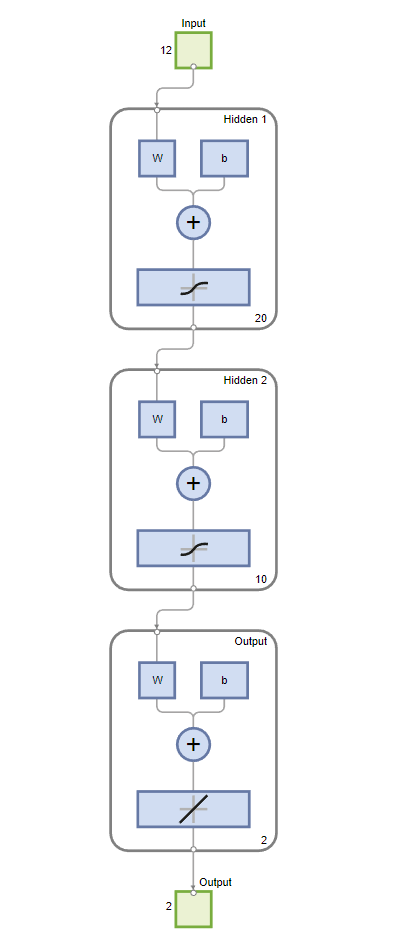
\includegraphics[width=0.25\textwidth]{figures/red.png}
	\end{figure}
	
	
	\subsection{Código}
	\inputminted[fontsize=\scriptsize, linenos, breaklines=true, xleftmargin=0.75cm, frame=lines]{matlab}{code/red,png}
    
        \subsection{i}
        
        \subsection{ii}
        
        \subsection{iii}
        
        \subsection{iv}
        
        \subsection{v}
        
    \section{b)}
    
    \section{c)}
    
    \section{d)}

                
    \part{Diseño automático de un controlador neuronal.}
	
    \section{Obtener los datos de entrenamiento}
        Para esta parte de la práctica en primera instancia se intentó recopilar los datos a partir del control manual, pero tras comprobar la falta de consistencia y la complejidad de hacerlo de este modo se decidió pasar a la siguiente opción proporcionada en el enunciado, \textquoteleft b) Realizar un recorrido prefijado \textquoteright \\
        
    	El código para la generación de los datos de entrenamiento está hecho a partir del proporcionado en el aula virtual de la asignatura, cambiando tras el mensaje de inicialización y la inicialización de la matriz training\_data. El primer cambio que aparece es un bucle que verifica la llegada de los mensajes de los sensores
    
        \inputminted[fontsize=\scriptsize, linenos, breaklines=true, xleftmargin=0.75cm, frame=lines, firstline=70, lastline=77]{matlab}{code/maniobra_park_ackerman_datos_entrenamiento_alumnos.m}
    
        Para entrenar la red de forma que pueda aparcar desde distintas posiciones de inicio, se han almacenado datos de diferentes aparcamientos exitosos con posiciones iniciales distintas. La siguiente parte del código son los valores de cada avance realizado por el vehículo en cada simulación. La elección de qué mapa utilizar está determinada por qué secciones se comentan o descomentan en el código.
    
        \inputminted[fontsize=\scriptsize, linenos, breaklines=true, xleftmargin=0.75cm, frame=lines, firstline=79, lastline=103]{matlab}{code/maniobra_park_ackerman_datos_entrenamiento_alumnos.m}
    
        Estos valores se aplican a la simulación igual que en el código proporcionado a los alumnos, con la diferencia de que se realiza en un bucle para jecutar los avances para cada conjunto de distancias, velocidades y ángulos en el mapa seleccionadoguardar los datos de todos los avances.
    
        \inputminted[fontsize=\scriptsize, linenos, breaklines=true, xleftmargin=0.75cm, frame=lines, firstline=104, lastline=110]{matlab}{code/maniobra_park_ackerman_datos_entrenamiento_alumnos.m}
    
        Tras la simulación se ha añadido una comprobación del éxito del aparcamiento, la cual se realiza manualmente, introduciendo el resultado con el teclado (una \textquoteleft s \textquoteright almacena los datos al final de la matriz training\_data.
    
        \inputminted[fontsize=\scriptsize, linenos, breaklines=true, xleftmargin=0.75cm, frame=lines, firstline=112, lastline=122]{matlab}{code/maniobra_park_ackerman_datos_entrenamiento_alumnos.m}
    
        Con este código se almacena en el archivo "datos\_training\_definitivo" la matriz training\_data con los datos recogidos de los 12 sónares, las velocidades y los ángulos del volante
    
    \section{Generar la red con la configuración deseada y preparar los datos de entrenamiento.}

        En el archivo \textquoteleft control\_neuronal.m \textquoteright, se establece la configuración de la red neuronal encargada de controlar el vehículo. Para lograr una red con la capacidad óptima para ejecutar la maniobra deseada, se procede a entrenar la red en un ciclo específico solo si su rendimiento ha caído por debajo de un umbral predefinido.\\
        En primer lugar, se inicializan las variables que determinan el número de ciclos y el umbral de rendimiento del entrenamiento, junto con una red neuronal inicial que cuenta con tres capas ocultas, cada una compuesta por 6, 7 y 6 neuronas, respectivamente.
    
        \inputminted[fontsize=\scriptsize, linenos, breaklines=true, xleftmargin=0.75cm, frame=lines, firstline=0, lastline=6]{matlab}{code/control_neuronal.m}
    
        Después comienza el bucle del entrenamiento, que se ejecuta una vez por cada ciclco de entrenamiento. Al principio del bucle, se desordenan las filas de la matriz training\_data con la que se entrena la red. Esto ayuda a mejorar la generalización del modelo al evitar que la red memorice el orden de los datos.

        \inputminted[fontsize=\scriptsize, linenos, breaklines=true, xleftmargin=0.75cm, frame=lines, firstline=8, lastline=12]{matlab}{code/control_neuronal.m}

        Entonces se crea una variable a partir de training\_data permutado con los datos que se van a usar, en nuestro caso todos los registros de todos los sónares como entradas y la velocidad y ángulo del volante como salidas. Los valores registrados como infinito se cambian a 5.0 en la línea 20 del código para que no afecten al entrenamiento.

        \inputminted[fontsize=\scriptsize, linenos, breaklines=true, xleftmargin=0.75cm, frame=lines, firstline=14, lastline=22]{matlab}{code/control_neuronal.m}

        La red a entrenar será una copia de la inicializada anteriormente, la cual la sustituirá en caso de cumplir con el umbral de entrenamiento. Se configura y entrena la red con los parámetros definidos anteriormente, se muestra por pantalla el rendimiento y, en caso de ser menor que el determinado al principio del código, se prosigue con el entrenamiento de la red. En caso contrario se descarta y se reinicia el bucle.

        \inputminted[fontsize=\scriptsize, linenos, breaklines=true, xleftmargin=0.75cm, frame=lines, firstline=28, lastline=48]{matlab}{code/control_neuronal.m}
        
    \section{Generar el bloque de simulink}

        Al terminar de entrenarse la red se genera el bloque de simulink que controlará el vehículo en la simulación.
    
        \inputminted[fontsize=\scriptsize, linenos, breaklines=true, xleftmargin=0.75cm, frame=lines, firstline=50, lastline=51]{matlab}{code/control_neuronal.m}
    
    \section{Modificar el diagrama de simulink}
	   
	El diagrama de simulink que contiene la red neuronal está guardado con el nombre \textquoteleft ackerman\_ROS\_controller\_neuronal.slx\textquoteright. En este diagrama se ha cambiado el controlador por el generado en el paso anterior y añadido el bloque \textquoteleft Data Type Conversion\textquoteright entre la salida del multiplexor de los ultrasonidos y la entrada de la red.

        \begin{figure}[htp!]
		\centering
		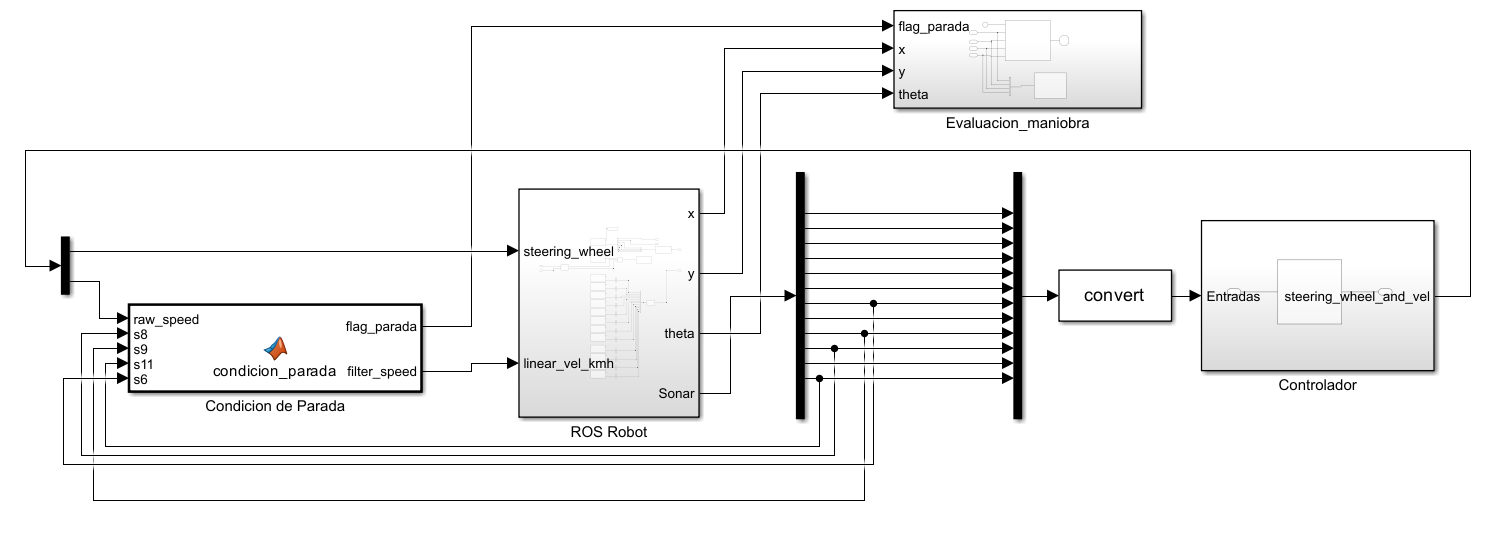
\includegraphics[width=1\textwidth]{PracticaFinal/figures/diagrama_simulink_neuronal.png}
	\end{figure}

        \subsection{Modificar la condición de parada}

            Dado que la red neuronal no regula la distancia a la pared como el control borroso, se ha modificado la condición de parada para obtener una posición más cercana a la ideal según el enunciado. Para esto se han conectado los datos de los sónar traseros y laterales (de la parte de atrás) y ajustado la condición de parada en función de estos.

            
 \end{document}
